\documentclass[12pt]{article}
\usepackage[utf8]{inputenc}
\usepackage[T1]{fontenc}
\usepackage{indentfirst}
\usepackage{amsmath}
\usepackage{amssymb}
\usepackage{natbib}
\usepackage{graphicx}
\usepackage{float}
\usepackage[a4paper, margin = 2 cm]{geometry}
\usepackage{fancyhdr}
\usepackage{wrapfig}
\usepackage{hyperref}

\title{JAiO zadanie 4}
\author{Dominik Wawszczak}
\date{2023-06-06}

\begin{document}
	\setlength{\parindent}{0 cm}
	
	Kacper Bal 439948 \hfill Zadanie 1
	
	Piotr Blinowski 439949
	
	Dominik Wawszczak 440014
	
	\bigskip
	\hrule
	\bigskip
	
	Udowodnimy, że język
	\[ L \ = \ \left( \left\{ a^{n} b^{n} \ : \ n \in \mathbb{Z}^{+} \cup
	\left\{ 0 \right\} \right\} \right) ^ {\ast} \]
	nie jest rozpoznowany przez żaden automat ze stosem pracujący w skończenie
	wielu fazach.
	
	\medskip
	
	Na początek udowodnimy, że \(L \in \text{CFL}\). Weźmy gramatykę
	\(\mathcal{G} = \left( \left\{ a, b \right\}, \left\{ S, T \right\}, P, S
	\right)\) z produkcjami:
	\begin{itemize}
		\item \(S \longrightarrow SS \mid T \mid \varepsilon\),
		\item \(T \longrightarrow aTb \mid \varepsilon\).
	\end{itemize}
	Łatwo widać, że gramatyka \(\mathcal{G}\) opisuje język \(L\), jednak nie
	będziemy zagłębiać się w szczegóły. Wynika z tego, że \(L \in \text{CFL}\).
	
	\medskip
	
	Przypuśćmy nie wprost, że istnieje automat ze stosem \(\mathcal{A}\) o
	zbiorze stanów \(Q\) i zbiorze symboli stosowych \(\Gamma\), działający w co
	najwyżej \(k\) fazach, rozpoznający język \(L\). Przez resztę rozwiązania
	zadania będziemy działać na słowie \(w = \left( a^{X} b^{X} \right) ^ {Y}
	\in L\), gdzie \(X = 21 \cdot \left| Q \right| \cdot \left| \Gamma \right| +
	37\), a \(Y = 69 \cdot k \cdot X + 420\).
	
	\medskip
	
	Wprowadźmy następujące definicje:
	\begin{itemize}
		\item \textit{długością} fazy nazwiemy liczbę przejść, które dana faza
		      zawiera, przy czym uwzględniamy tutaj zarówno przejścia po
		      literach czytanego słowa, jak i \(\varepsilon\)-przejścia;
		\item \textit{zmianą} fazy nazwiemy wartość bezwzględną różnicy rozmiaru
		      stosu na początku i na końcu fazy.
	\end{itemize}
	
	\medskip
	
	\textbf{Lemat 1}
	
	
	
	W biegu akceptującym automatu \(\mathcal{A}\) po słowie \(w\), w ramach
	jednej fazy nie może być ciągu \(\left| Q \right|\) kolejnych przejść
	niezmieniających stosu.
	
	\medskip
	
	\textbf{Dowód Lematu 1}
	
	Przypuśćmy nie wprost, że w pewnej fazie wystąpiło \(\left| Q \right|\)
	kolejnych przejść niezmieniających stosu. Wówczas z Zasady Szufladkowej
	Dirichleta wynika, że wśród tych przejść pewien stan \(q\) wystąpił co
	najmniej \(2\) razy, ponieważ łącznie automat przeszedł przez \(\left| Q
	\right| + 1\) stanów. Jeśli od pierwszego do drugiego znalezienia się w
	stanie \(q\) automat wykonał same \(\varepsilon\)-przejścia, to nie miały
	one sensu, ponieważ nic się nie zmieniło, możemy więc założyć, że słowo
	wczytane w tym okresie jest niepuste. Łatwo widać, że słowo to można
	napompować, a ponieważ ma ono długość co najwyżej \(\left| Q \right|\), to z
	pewnością nie jest ono postaci \(\left( a^{X} b^{X} \right) ^ m\), dla
	pewnego \(m \in \mathbb{Z}^{+}\), zatem na skutek tego pompowanie powstanie
	nowe słowo nienależące do \(L\), po którym będzie istniał bieg akceptujący
	automatu \(\mathcal{A}\). Otrzymana sprzeczność końćzy dowód lematu.
	
	\medskip
	
	\textbf{Lemat 2}
	
	\[ \text{Jeśli faza ma długość} \ n
	\text{, to jej zmiana należy do przedziału} \ \left[ \left\lfloor
	\frac{n}{\left| Q \right|} \right\rfloor, n \right] \text{.} \]
	Lemat ten jest bezpośrednim wnioskiem z lematu 1.
	
	\medskip
	
	Zauważmy, że w biegu akceptującym automatu \(\mathcal{A}\) po słowie \(w\)
	musi istnieć faza push długości co najmniej \(3X\), co wynika z doboru
	stałej \(Y\), ponieważ w przeciwnym wypadku z lematu 2 musiałby być wykonany
	pop na pustym stosie. W trakcie tej fazy wczytany więc zostanie pełny blok
	\(b^{X}\). Z doboru stałej \(X\) oraz Zasady Szufladkowej Dirichleta wynika,
	że w trakcie przechodzenia tej fazy przez blok \(b^{X}\) dwa razy wystąpi
	moment, że aktualny stan to pewne \(q\), a aktualny symbol na szczycie stosu
	to pewne \(s\). Ponownie, wczytane słowo pomiędzy tymi dwoma momentami jest
	niepuste, a dodatkowo ma długość co najwyżej \(\left| Q \right| \cdot \left|
	\Gamma \right|\). Stos natomiast powiększy się o pewne słowo \(v\) długości
	również co najwyżej \(\left| Q \right| \cdot \left| \Gamma \right|\),
	którego ostatnia litera to oczywiście \(s\).
	\begin{center}
		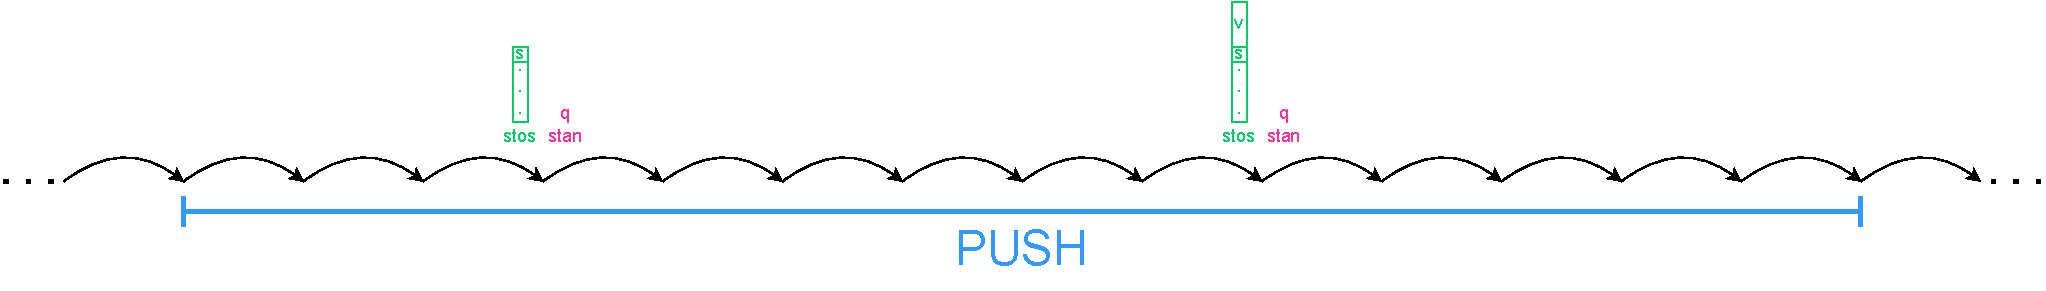
\includegraphics[width = 0.9 \textwidth]{./image-1.pdf}
	\end{center}
	
	\medskip
	
	Chcemy teraz podwoić fragment przeczytany pomiędzy dwoma opisanymi w
	poprzednim akapicie momentami. Oczywiście skutkiem takiego podwojenia będzie
	uzyskanie nowego słowa \(w' \notin L\). Rozważmy dwa przypadki:
	\begin{enumerate}
		\item Symbol \(s\) do końca biegu automatu pozostaje na stosie.
		      
		      Łatwo wówczas zauważyć, że słowo \(w'\) zostanie zwyczajnie
		      zaakceptowane przez automat \(\mathcal{A}\), ponieważ podwojony
		      fragment dopisuje tylko słowo \(v\) do stosu, a skoro litera
		      bezpośrednio pod tym słowem nie zostanie zdjęta, to z perspektywy
		      automatu nie będzie różnicy.
		
		\item W przeciwnym wypadku, w dalszej części biegu automatu istnieje
		      spójny fragment ciągu przejść odpowiadający za zdjecie ze stosu
		      słowa \(v\). Bardziej formalnie, na początku tego ciągu stos jest
		      postaci \(pref \cdot v\), a na koniec po prostu \(pref\). W
		      trakcie natomiast na stosie mogą być wykonywane zarówno operacji
		      push, jak i pop. Zmodyfikujmy słowo \(w'\) tak, aby ten drugi
		      fragment również był podwojony. Słowo to dalej nie należy do
		      języka \(L\), ponieważ nie zgadza się liczba liter \(b\) w tym
		      pierwszym podwojonym fragmencie (w drugim może być cokolwiek,
		      istotne jest to, że występuje on później). Tak jak w poprzednim
		      przypadku, z perspektywy automatu nie będzie różnicy i ponownie
		      będzie wykonywał takie przejścia jak w biegu akceptującym po
		      słowie \(w\), w oparciu jedynie o aktualny stan, aktualną literę i
		      aktualny symbol na szczycie stosu.
	\end{enumerate}
	
	\medskip
	
	Z powyższego wynika, że automaty ze stosem pracujące w skończenie wielu
	fazach nie rozpoznają wszystkich języków bezkontekstowych (w szczególności
	\(L\)), co kończy rozwiązanie zadania.
	\begin{flushright}
		\(\Box\)
	\end{flushright}
\end{document}
